\documentclass[11pt,a4paper]{article}

\usepackage[debug, coloredLinks=false, langue=american, bibStyle=apa]{pages/preambules/preambule}	


% \newglossaryentry{<label>}{
%	 name = {<nom>},
%	 description = {<description>},
%	 first = {<premier appel>},
%	 plural = {<si on ajoute pas de 's' à la fin>},
%	 symbol = {<symbole pi>},
% 	 see = {<label_a_voir},
% }

% \newacronym{<label>}{<abbreviation>}{<full>}
% \newacronym[longplural={pluriel}]{<label>}{<abbreviation>}{<full>}


% utilisation (pour tout):
% - \gls(<label>)
% - \Gls(<label>)  		=> avec majuscule
% - \glspl(<label>)  	=> pluriel
% - \Glspl(<label>)		=> pluriel avec majuscule
% - \glsdesc{<label>}  	=> affiche la description
% - \glssymbol{<label>}	=> affiche le symbole

% utilisation en plus pour les accronymes : 
% - \acrshort{<label>}	=> donne l'abbréviation
% - \acrlong{<label>}	=> donne la description "full"
% - \acrfull{<label>}	=> donne "full (abbreviation)"



\newglossaryentry{mot}{
	name=mot,
	description={un mot},
	first={le premier mot (mot))}
}
	
\addbibresource{pages/bibliographie/bibliographie.bib}
% https://en.wikibooks.org/wiki/LaTeX/Bibliography_Management#biblatex


\lfoot{\em Polytech Nantes, Computer Science Department} 


\begin{document}

\pagestyle{fancy}		% on remet le header et footer
\pagenumbering{arabic} 	% numérotation 1, 2, 3


\begin{titlepage}	% Pour réaliser une page de couverture

\begin{center}


% images en haut de page
\begin{minipage}[t]{0.48\textwidth}
	\begin{flushleft}
		
\includegraphics [width=60mm]{images/logo_ecoles/Polytech_Nantes_Universite} \\[0.5cm]
	\end{flushleft}
\end{minipage}
\begin{minipage}[t]{0.48\textwidth}
	\begin{flushright}
		
\includegraphics [width=60mm]{images/upes} \\[0.5cm]
		%\textsc{\LARGE Entreprise}
	\end{flushright}
\end{minipage} 

\vfill

\Huge{\textbf{4$^{th}$ year Internship report}} \\
\huge{\textbf{3D Map generation and autonomous navigation using Symbolic Computing}}

\vfill 

\Large{\textbf{Synopsis}} 

\vfill

\Large{\textbf{Handed over}} \\
%\LARGE{\textbf{Polytech Nantes\\Graduate school of Engineering of the University of Nantes\\Computer Science Department}}  
\LARGE{\textbf{University of Petroleum and Energy Studies}}

\vfill 

\Large{Carried out by} \\
\Large{\textbf{Maxime PINEAU}} 

\vfill 

%\Large{\textbf{SOUS LA DIRECTION DE}}\\
%\Large{\textbf{Monsieur xxx XXX}} 

\Large{Under the direction of} \\
\Large{\textbf{Doctor Niharika SINGH}} 

\vfill


%\Large{\textbf{Entreprise d'accueil}} \\
%\LARGE{\textbf{ENTREPRISE} }\\
%\Large{\textbf{ADRESSE}} 


%\Large{\textbf{Du 6 Juillet 2015 au 1 Août 2015\\(4 semaines)}} 

\Large{From 30th May 2016 to 26 August 2016}

\vfill

\large{Version of} \\
\large{\today} 

\vfill


\includegraphics[scale=0.6]{images/logo_ecoles/Universite_de_Nantes_} 

\vfill

\large{2015 - 2016} 



%\large{\textbf{D\'{E}PARTEMENT INFORMATIQUE}}\\
%\Large{\textbf{INSTITUT UNIVERSITAIRE DE TECHNOLOGIE}}\\
%\large{\textbf{NANTES - FRANCE}}
%\large{\textbf{\\2013-2014}}\\[0.5cm]
%
\includegraphics[scale=1.4]{images/logo_ecoles/Universite_de_Nantes_}\\


\end{center}

\end{titlepage}

\tableofcontents 

\section{Abstract}
% le problème à résoudre


This project involves moving an autonomous robot in an unknown environment, with a minimum of time and energy concuption. For example, the robot will have to explore and search into an unknown environment, such as a the planet Mars or a submarin field. An autonomus robot could be used in differents domains, such as  surveillance (drones), transport, or cleaning. The robot will have to generate a 3D map of his surrounding, take a decision accordingly, move and then learn from this decision. The robot will use reinforcment learning to learn from his previous decisions. As for the generation of the 3D map, we will be using \gls{DEM} and Symbolic Computing. 

~~

\textbf{keywords :} 3D Map Generation, Autonomous Navigation, DEM, Symbolic Computing, STRT 


\section{Aim and Objectives}
% qu'est ce qu'on va faire pour résoudre ce problème 

In order to generate the 3D map, we will use \gls{DEM}, Symbolic Computing and a \gls{CLAP} algorithm (which is used for image processing and pattern recognition). The \gls{DEM} images will have to be transform with a \gls{STRT}, a tranformation involving Symbolic Computing. Nowadays 3D map generation technologies generally use DIP methods, but \gls{DEM} method was selected because it is faster during the compilation time. 


In order to visualize the effects of the differents techniques we will use, we will develop a \gls{GUI} where each steps could be done separately. The user will have to charge an image and apply a transformation on it by selecting one. A new image will be generated, with the name of the operation and the time it has taken to process. 


The reinforment learning algorithm, which will allow the robot to self-learning through experiences, will use a reward policy. 


As the University doesn't have the actual robot for the moment, this project will be conduct under a simulated environnement. 


\section{Introduction}
% les topiques 

The robot will be equiped by differents camera, allowing it to take pictures from different angles. Those pictures, or input images, correspond to the surrounding of the robot. It will also be equiped with differents sensors that will provide additionnal information, such as depth, hight or spacial position (x, y, z). As the University doesn't have a robot yet, those pictures will be provided by the University. 

~~

After having those input images, the robot will have to : 
\begin{enumerate}
	\item process the input images of his surrounding, in order to create a \gls{DEM} 
	\item generate the 3D map by analysing the \gls{DEM} 
	\item analyse this 3D map and take a decision (knowing his previous decisions, if they exist), it will decide were to go
	\item analyse his decision, and learn from it 
\end{enumerate}


\begin{figure}[H]
	\centering
	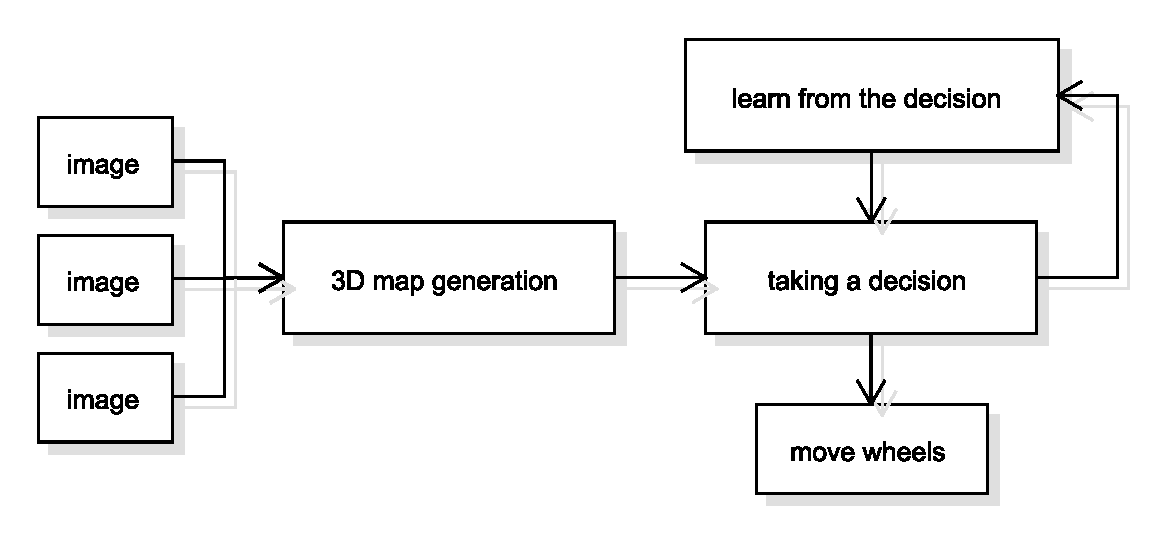
\includegraphics[width=0.7\textwidth]{images/diagrammes/flowchart_general}
	\caption{General functioning}
	\label{fig:diagram:general functioning}	
\end{figure}

The following sections will present the \gls{DEM} generation and the technics we will use in order to perform it. 


\subsection{DEM generation}

The first part of the process will be handeling the input images and apply a \gls{STRT} on them. So the \gls{STRT} would work, it is important to have $2^{k}$ number of pixels in each images. By performing a \gls{STRT} and a \gls{ISTRT} on one image, we will get a filtered image, with less noise.

~~ 

After the noise has been removed from all of the image, we will detect eadges on it by  transformng the image into a monochrome image (with only 2 values, 1 and 0) and apply a eadge detection algoritm. 

~~ 

By detecting the eadges, we will be able to identify each objects on the image, and extract those objects. 



\subsection{Rajan Transformation and it's application in the sets }

In this section, we will present the forward rajan transfom and it's application in the set domain. The reverse transforms won't be presented. Every equations, figures and explainations have been inspired by the following reference  \cite{bib:rajan_transformation}.


\subsubsection{Rajan Transformation}

The rajan transform take a sequence of $2^{i}$ numbers (the number of element of the sequence have to be a power of 2), transform it, and return another sequence of $2^{k}$ numbers. We will call $x(k)$ the input sequence, $X(k)$ the output sequence of the tranform, and $N$ the number of element in the sequence \cite{bib:rajan_transformation}. 

\begin{equation}
x = x(0), x(2), \cdots, x(k-1) \text{ where k is a power of 2}
\end{equation}

We will define two other sequences $g(k)$ and $h(k)$ as following : 
\begin{equation}
g(k) = x(k) + x(k + \frac{N}{2}) \text{ with } 0 \leq k \leq \frac{N}{2}
\end{equation}

\begin{equation}
h(k) = | x(k) - x(k - \frac{N}{2}) | \text{ with } \frac{N}{2} \leq k \leq N
\end{equation}


In other words, the sequence $x$ will be divided in two. Then we will sum the two first value of the subsequences (which will give us the results of $g(1)$), then the two seconds values (which is $g(2)$), then the thirds values, and so on until all the elements were processed. Then we will do the same operations but with a substraction instead (to get the sequence $h$).

~~

This processus will then have to be repeated on the subsequences $g$ and $h$ separately. We can see here the recursive character of this transformation. The figure \ref{fig:diagram:rajan transform} illustrate the rajan tranformation in a more procedural way, with a sequence of 4 elements. 

\begin{figure}[H]
	\centering
	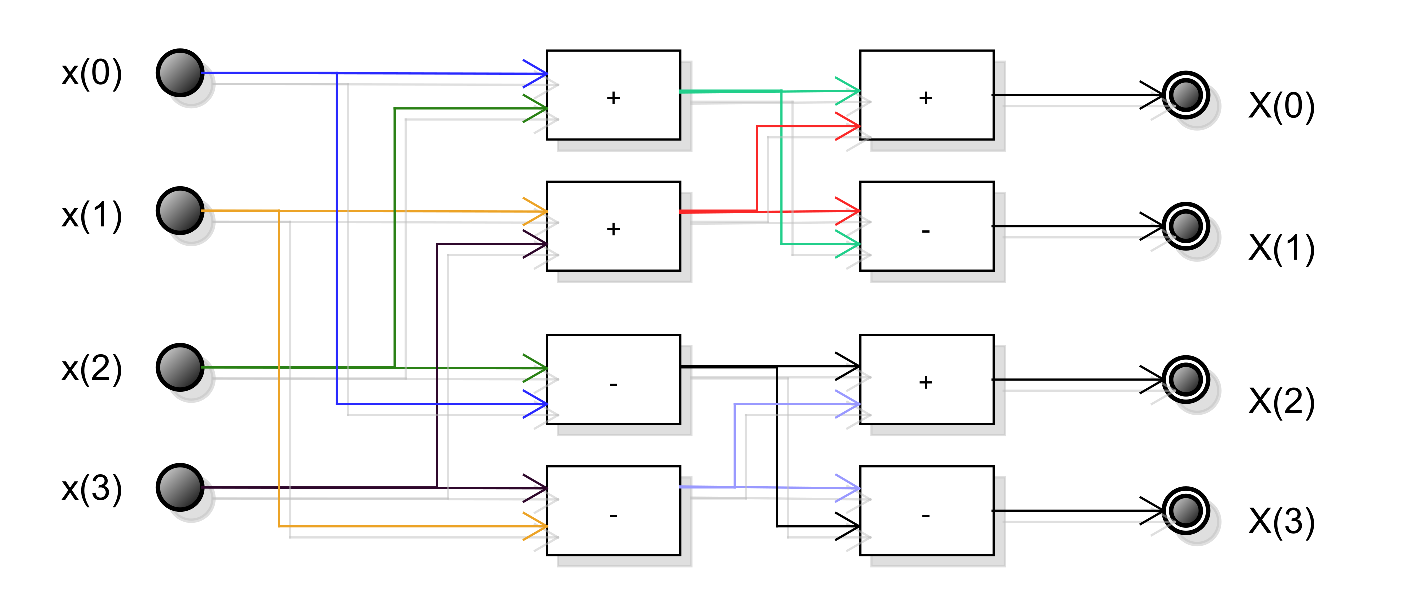
\includegraphics[width=0.7\textwidth]{images/diagrammes/rajan_transform}
	\caption{The forward Rajan Tranfform (RT)}
	\label{fig:diagram:rajan transform}	
\end{figure}



\subsubsection{Set Theoretic Rajan Transformation}

The set theoretic rajan transform is the application of the rajan transform in the set domain, and so instead of tranforming a sequence of numbers, it will tranform a sequence of sets, and return another sequence of sets. 

~~

In the set domain, the addition correspond to the union, and the substraction to the difference of two sets.



\section{Methodology}
% comment je vais le faire (lire doc, comprendre les techno, écrire algo, implémenter, documenter)

I am planning to divise this work into 3 parts, which will concern : 
\begin{enumerate} 
	\item the DEM generation (which involves Symbolic Computing, and STRT)
	\item the 3D Map Generation 
	\item the Autonomous Navigation and the Renforcement Learning 
\end{enumerate}

During each part, I will document myself on the subject, then write an algorithm, implement it, and finally document my work. 


\printbibliography
\printglossaries

\end{document}